\documentclass{article}

% for images: png, pdf, etc
\usepackage{graphicx}

% for nice table formatting, i.e. /toprule, /midrule, etc
\usepackage{booktabs}

% to allow for \verb++ declarations in captions.
\usepackage{cprotect}

% for nice source code syntax highlighting, also provides Listing env
%\usepackage{minted}

% for nice units
\usepackage{siunitx}

% for less margin space
%\usepackage{fullpage}

% for nice todo notes
\usepackage{todonotes}

% macros
\newcommand{\mstar}{\mathbf{m}^*(\varphi)}
\newcommand{\K}{\mathbf{K}(\varphi)}

\author{Jason K. Moore and Antonie van den Bogert}

\title{Direct Control Identification in Human Gait}
\title{Directly Identified Gait Phase Scheduled Feedback Gains Exhibit Positive
  and Negative Feedback}

\date{}

\begin{document}

\maketitle

\section*{TODO}

\listoftodos

\begin{abstract}
  \todo[inline]{Write one!}
\end{abstract}

\section*{Introduction}
%
Recent research and commercial activity indicate that gait-related powered
prosthetics will play an important role in both assisting humans with
disabilities and enhancing the abilities of the able bodied. These devices
include a variety of sensors and actuators than can be coupled to a control
system to provide acutated gait assistance. However, for example, the available
lightweight lower extremity exoskeletons lack gait that resembles an
able-bodied human both in terms of stability and ``natural'' gait motions.

Given a ``human-like'' system, i.e. one with similar degrees of freedom and
inertial properties to a human, that is actuated with simple joint torques can
we identify a feedback control mechanism for this system that causes it to
walk stably and recover from perturbations in much the same way a human does?

We hypothesize that typical gait measurements taken while a person is
walking under the influence of perturbations can be used to identify a
feedback controller for a similar system.

It is difficult to design a controller from first principles
for this very non-linear system. Although work based on \cite{Geyer2010} are
giving promising results in simulated musculoskeletal systems \cite{Wang2010,
Geitenbeek2014}. Even though constraining the controller to rudimentary models
of the muscoulo skeleteal system is fruitful, we are curious if more generic
black box control models can reveal more robust controllers. To improve the
gait of powered prosthetics, our intent is to identify a simple, linear
controller from a large set of data collected from able-bodied subjects being
perturbed by random longitudinal forces.

There are other researchers thinking along these lines. Elliot Rouse identified
the parameters of a linear model of the ankle's passive and active stiffness
and damping by perturbing around 400 stance phases of the gait cycle and
fitting a model with linear least squares. \cite{Wang2013} are able to predict
foot placement with a simple linear model derived from kinematic data that
relates the mid-stance pelvic state with the following foot location. Neither
of these explicitly tease out the feedback mechanism.

We answer this question by collecting greater than 15,000 gait cycles from 11
subjects walking at three nominal speeds on an instrumented treadmill where we
measure the kinematics of a full body marker set and a full set of ground
reaction loads at each foot while perturbing the subject by varying the belt
speed. We then identify a gait phase gain scheduled non-linear controller with
the direct identification method~\cite{Ljung1999}.

\section*{Methods}
%
\subsection*{Experiments}
%
We make use of a subset of the gait data reported in \cite{Moore2015} and refer
the reader to that publication for the details about the experiments and data.
The subset of the data includes a large number of gait cycles for 11 subjects
subjects walking at three nominal speeds on a treadmill with and without
pseudo-random longitudinal perturbations, i.e fluctuations in the belt speed.
The subject metadata parameters are given in Table~\ref{tab:subjects}.
%
\begin{table}
  \cprotect\caption{Information about the 11 study participants. The final
    three columns provide the trial numbers associated with each nominal
    treadmill speed. The measured mass is computed from the mean total vertical
    ground reaction force just after the calibration pose event. Generated by
    \verb|src/subject_table.py|.}
  \centering
  \begin{tabular}{rlrrrrrr}
\toprule
 Id &  Gender &  Age [yr] & Height [m] &                     Mass [kg] & 0.8 m/s & 1.2 m/s & 1.6 m/s \\
\midrule
    &         &           &            &                               &         &         &         \\
  3 &  female &        32 &       1.62 &      $54\pm2$ &      46 &      47 &      48 \\
  5 &    male &        23 &       1.73 &  $71.2\pm0.9$ &      32 &      31 &      33 \\
  6 &    male &        26 &       1.77 &  $86.8\pm0.6$ &      40 &      41 &      42 \\
  7 &  female &        29 &       1.72 &  $64.5\pm0.8$ &      16 &      17 &      18 \\
  8 &    male &        20 &       1.57 &  $74.9\pm0.9$ &      19 &      20 &      21 \\
 10 &    male &        19 &       1.77 &      $92\pm2$ &      61 &      62 &      63 \\
 12 &    male &        22 &       1.85 &  $74.2\pm0.5$ &      49 &      50 &      51 \\
 13 &  female &        21 &       1.70 &      $58\pm2$ &      55 &      56 &      57 \\
 15 &    male &        22 &       1.83 &  $80.5\pm0.8$ &      67 &      68 &      69 \\
 16 &  female &        28 &       1.69 &  $56.2\pm0.6$ &      76 &      77 &      78 \\
 17 &    male &        23 &       1.86 &  $88.3\pm0.8$ &      73 &      74 &      75 \\
\bottomrule
\end{tabular}

  \label{tab:subjects}
\end{table}

\subsection*{Data Preprocessing}
%
The ``raw'' data provided by \cite{Moore2015} consists of 100~\si{\hertz} time
series of marker and ground reaction loads in addition to event time
identifiers. We make use of an open source software package,
GaitAnalysisToolKit, to process the data. The processing follows these steps:
%
\begin{enumerate}
  \item Identify missing markers and the corresponding time instances.
  \item Replace missing markers with linearly interpolated values.
  \item Filter all signals with a forward/backward 2nd order low pass
    Butterworth filter with a cutoff frequency of 6~\si{\hertz}.
  \item Section the trials into unperturbed and perturbed sections based on the
    event times.
  \item Compute the planar inverse dynamics for the lower body: right and left
    ankle, knee, hip joint angles, joint angular rates, and joint torques.
  \item Identify the heelstrike times based on the vertical ground reaction
    force.
  \item Segment the time series into gait cycles based on the right foot's
    heelstrikes.
  \item Linearly interpolate the time series in each gait cycle to a specific
    number of data points so all gait cycles have the same number of samples.
  \item Remove any outlier gait cycles that were not properly identified due to
    abnormal ground reaction force measurements.
\end{enumerate}

After the initial processing above, the data is stored in three dimensional
arrays M x N x (q + p), where M is the number of gait cycles, N is the number of time
instances in the gait cycle, and (q + p) are the number of measurements.
Figure~\ref{fig:angle-torque-comparison} shows the mean and standard deviation
of across the gait cycles for selected time series for both unperturbed and
perturbed walking. Furthermore, Figure~\ref{fig:gait-cycle-stats-comparison}
compares several gait statistics of interest for unperturbed and perturbed
walking. These two figures are intended to show that there is variation in the
subject's motion that is a direct result of the longitudinal perturbations.
%
\begin{figure}
  \centering
  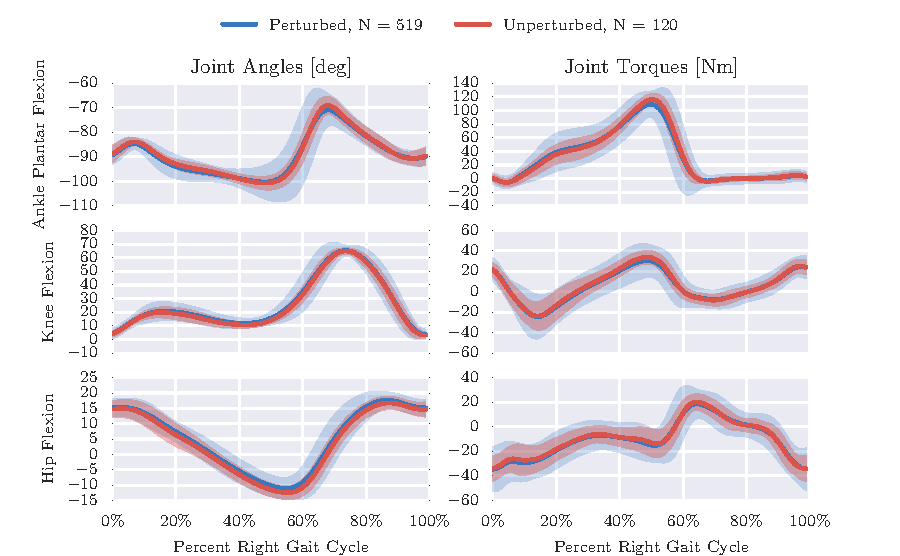
\includegraphics{figures/unperturbed-perturbed-comparison.pdf}
  \cprotect\caption{Right leg mean and $3\sigma$ (shaded) joint angles and
    torques from both unperturbed (red) and perturbed (blue) gait cycles
    from trial 20. We define the nominal configuration, i.e. all joint angles
    equal to zero, such that the vectors from the shoulder to the hip, the hip
    to the knee, the knee to the ankle, and the heel to the toe are all aligned.
    Produced by \verb|src/unperturbed_perturbed_comparison.py|.}
  \label{fig:angle-torque-comparison}
\end{figure}
%
\begin{figure}
  \centering
  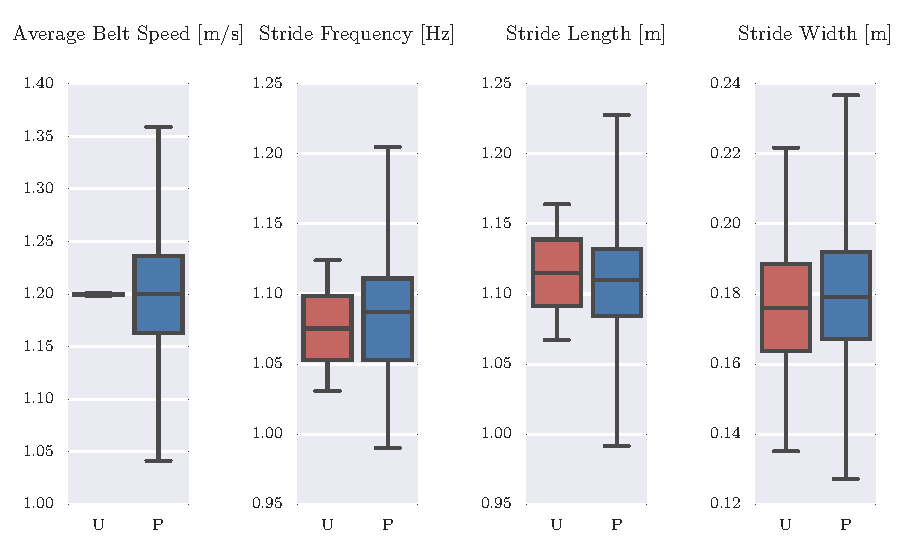
\includegraphics{figures/unperturbed-perturbed-boxplot-comparison.pdf}
  % NOTE : Make sure to update these values (120, 519) if anything in the
  % script changes.
  \cprotect\caption{Box plots of the average belt speed, stride frequency,
    stride length, and stride width which compare 120 unperturbed (U: red) and
    519 perturbed (P: blue) gait cycles. The median is given with the box
    bounding the first and third quartiles and the whiskers bound the range of
    the data. Produced by \verb|src/unperturbed_perturbed_comparison.py|.}
  \label{fig:gait-cycle-stats-comparison}
\end{figure}

\subsection*{Controller}
\label{sec:controller}
%
We assume a black box~\footnote{black box in the system identification sense,
i.e. there are parameters in the model} control structure for the closed loop
system, Figure~\ref{fig:controller}. We first assume there is an unknown
non-linear plant, i.e. the open loop musculoskeletal system and treadmill, that
has an uknown time varying state. This plant can be perturbed by an external
exogenous input $w(t)$, in our case by varying belt speed, and is also driven
by joint torques $\mathbf{m}(t)$. An unknown sensor model generates feedback
signals, $\mathbf{s}(t)$, that are compared to a nomimal gait phase dependent
reference trajectory $\mathbf{s}_0(\varphi)$ that describes the gait phase
varying state for cyclic gait when no feedback is necessary. The error in these
sensors are fed into the controller which generate corrective joint torques
that are added to the nomimal gait phase dependent joint torques
$\mathbf{m}_0(\varphi)$ that correspond to the nominal trajectories,
$\mathbf{s}_0(\varphi)$. We then assume that when the actual state deviates
from the nominal state trajectory that the controller computes additive joint
torques based on the state tractory error to compensate for variation in gait
away from the nomimal.

The controller is designated as a gait phase scheduled gain matrix, $\K$, that
relates the error in the state trajectories to the additive joint torques. The
controller structure bounded by the box in Figure~\ref{fig:controller} can be
described by the following algebraic equation.
%
\begin{equation}
  \mathbf{m}(t) = \mathbf{m}_0(\varphi) + \mathbf{K}(\varphi) [\mathbf{s}_0(\varphi) - \mathbf{s}(t)]
  \label{eq:controller}
\end{equation}
%
\begin{figure}
  \centering
  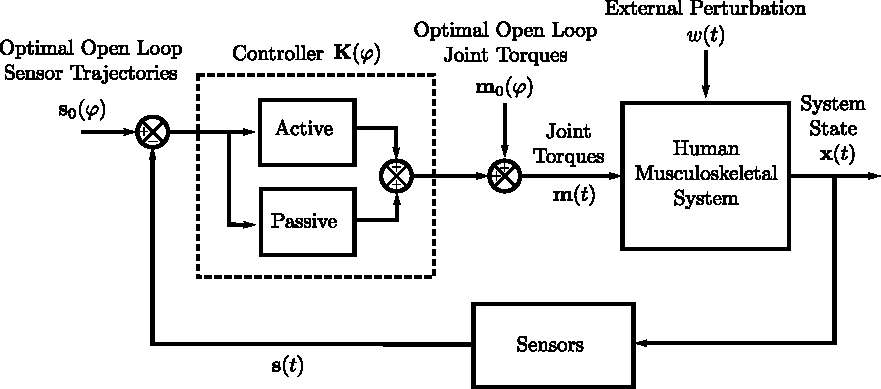
\includegraphics{figures/control-system.pdf}
  \caption{The controller block diagram}
  \label{fig:controller}
\end{figure}

It is important to note that this control structure will effectively lump the
passive control gains with the active ones in addition to any other unmodeled
effects. This is desirable for our intentions, as we are only concerned with
mapping this identified controller to that of powered prosthetic device and it
is thuse unnessary to distinguish between these.

\subsection*{Direct Identification}
%
We employ a direct identification approach to find the optimal parameters for
the control structure described in Section~\ref{sec:controller}. We are aware
that direct identifcation has its drawbacks. It is well known that process
noise due to unmodeled affects in the identification model will bias the
results towards the inverse of the plant if the external perturbations are not
sufficiently large enough~\cite{Ljung1999,Kearney1990,Kooij2005}. Determining
if the perturbations are of large enough size is difficult because the process
noise is generally unknown.

\todo[inline]{I need to explain why we think our perturbations may be large
  enough in magnitude. The problem is that we get similiar identification
  results from both unpertrubed and perturbed data. THis can mean one of two
  things: (1) the person perturbs themselves enough and the identification is
  correct either way or (2) our perturbations are not enough, i.e. we'd get
  different results by perturbing more. The only thing that I can think of here
  is to show the necessary perturbation level for the quiet standing case and
  then say that we have similar magnitudes.}

We reformulate Equation~\ref{eq:controller} to make it amenable to linear
identifaction. The equation can be rewritten so that is linear in the gains and
a new term $\mathbf{m}^*$.
%
\begin{equation}
  \mathbf{m}(t) = \mathbf{m}^*(\varphi) - \mathbf{K}(\varphi) \mathbf{s}(t)
  \label{eq:linear-form}
\end{equation}
%
where
%
\begin{equation}
  \mathbf{m}^*(\varphi) = \mathbf{m}_0(\varphi) + \mathbf{K}(\varphi) \mathbf{s}_0(\varphi)
\end{equation}

Assuming that we can collect noisy measurements of $\mathbf{m}(t)$
and $\mathbf{s}(t)$, $\mathbf{m}^*(\varphi)$ and $\mathbf{K}(\varphi)$ are
identified simply by using linear least squares to regress the data. Given $m$
gait cycles with $n$ time steps in each gait cycle with $q$ controls and $p$
sensors there are $nq(p + 1)$ unknowns and $mnq$ equations so we need at least
$p + 1$ gait cycles to solve for the unknowns.

Details of coercing Equation~\ref{eq:linear-form} into the canonical form,
$\mathbf{Ax}=\mathbf{b}$ can be found in the supplementary IPython notebook
\verb|form_linear_system.ipynb|.

We compute the scheduled gains and $\mathbf{m}^*$ for both the unperturbed and
perturbed gait cycles for each trial. Three quarters of the data from each
series of gait cycles are used to compute the unknowns and the model is
validated against the remaining one quarter of the data. We compute the
percentatge of variance accounted for by the model with respect to the
validation data set to gauage how well the model predicts.

\begin{equation}
  \textrm{VAF} = 1 - \frac{||\mathbf{m}_p - \mathbf{m}_m||}
    {||\mathbf{m}_m - \bar{\mathbf{m}}_m||}
  \label{eq:vaf}
\end{equation}

\section*{Results}
%
The formulation above allows one to choose a variety of combinations of
potential sensor, $\mathbf{s}(t)$, and actuator, $\mathbf{m}(t)$, signals to
generate a controller. For this analyses we assume we are constructing a
controller for a planar robot that involves the hip, knee, and ankle joints.
The angle and angular rate of each joint are available as sensors and a torque
at each joint are available as the actuators.

The most general case for the controller, $\K$, has q x p
unknown entries. The formulation allows for different types of control that
isolate actuators from sensors. We explore four of th

\begin{description}
  \item[Full Control] The torque genderated by a joint is affected by all of
    the available sensors.
  \item[Side Isolated Control] The torque generated at a joint is only affected
    by the sensors on the same side of the body.
  \item[Joint Isolated Control] The torque generated by a joint is only
    affected by the sensors that give information about that joint.
  \item[No Feedback Control] The motion is only governed by $\mstar$.
    \todo{Isn't the ``no feedback'' equivalent to $\mstar$ being equivalent to
    the mean torques?}
\end{description}

\subsection*{Example Result}
%
Once a controller is identified for a section of a trial the primary results of
interest are the gain values and how they change with respect to the gait phase
and then how well the model can predict the gait of the indepedent validation
data. The actual gain values may give some insight to the physiological nature
of the feedback mechanism. Here we present a typical result from a join
isolated controller structure. Figure~\ref{fig:example-gains} \todo{Explain the
shaded area: variance with respect to the fit.} shows the estimates of the
scheduled gains with respect to the percent gait cycle in each leg as a
function of the phase of the gait cycle. The top row of graphs show the
proportional gains, the middle row provides reference mean trajectories of the
sensor measurements, and the final row shows the derivative gains. Gains values
greater than zero indicate negative feedback and gains below zero indicate
positive feedback. \todo{The mismatch from positive feedback to negative K
values is potetnially confusing, as Ton has pointed out before, but to me this
is the standard way to describe a feedback system in control literature.}
%
\begin{figure}
  \begin{center}
    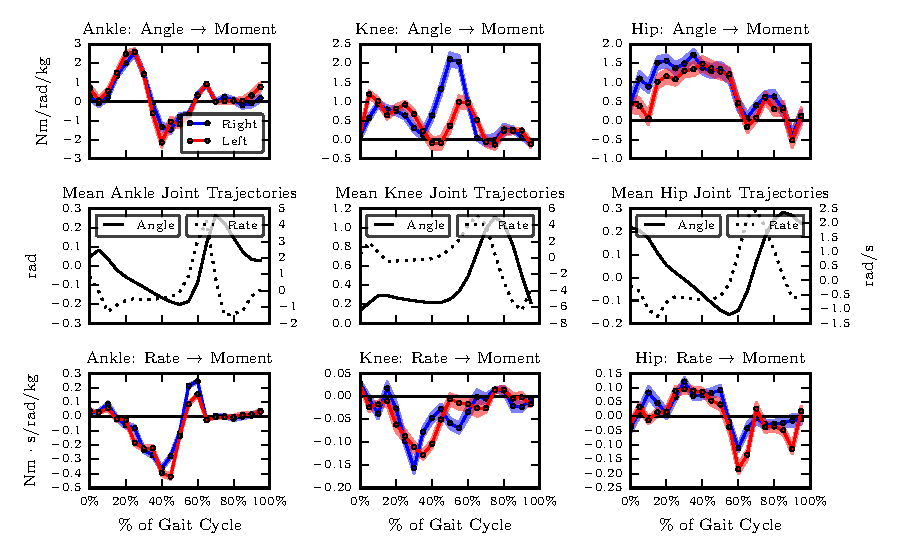
\includegraphics{figures/example-identified-joint-isolated-gains.pdf}
    \caption{Gait phase scheduled gains for the right (blue) and left
      (red) legs.}
    \label{fig:example-gains}
  \end{center}
\end{figure}

Figure~\ref{fig:example-fit} shows an example prediction of the measured ankle
plantarflexion torque in the right leg by the identified control model. The VAF
is reported for the entire validation period whereas only a select number of
gait cycles are shown. \todo{This plot technically shows the VAF based on the
20 samples per cycle comparison, yet I plot all of the measured values, i.e.
more like 100-120 samples per cycle.}
%
\begin{figure}
  \begin{center}
    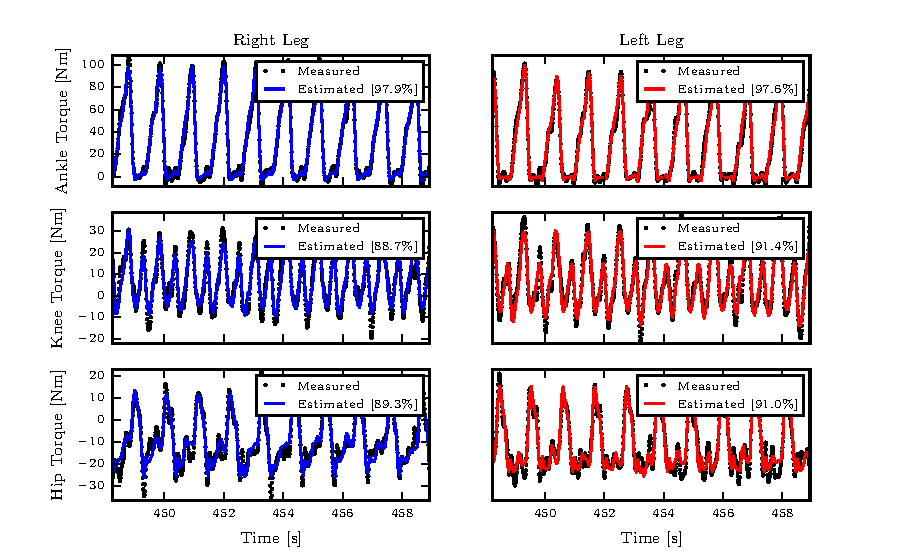
\includegraphics{figures/example-identified-joint-isolated-fit.pdf}
    \caption{Predicted torque compared to independent validation data.}
    \label{fig:example-fit}
  \end{center}
\end{figure}

\subsection*{Gains are consistent across subjects}
%
We compute the body mass normalized gains, $\frac{\mathbf{K}(\varphi)}{m}$ for
each subject at each nominal speed and examine the mean and standard deviation
across subjects for the inter-subject differences.
Figure~\ref{fig:mean-gains-1-2} shows the mean and standard deviation of the
gains identified from a joint isolated control structure at the
1.2~\si{\meter\per\second} nominal speed.
%
\begin{figure}
  \begin{center}
    \includegraphics{figures/example-mean-gains-1-2.pdf}
    \caption{Fill me in.}
    \label{fig:mean-gains-1-2}
  \end{center}
\end{figure}

The gains exhibit similar patterns, albeit with relatively large standard
deviations, across subjects. The differences in left and right sides are even
constant

\subsection*{Gains exhibit anatomical symmetry}
%

\subsection{Directly Identified Gait Phase Scheduled Feedback Gains Exhibit Positive
  and Negative Feedback}
%

\subsection*{Random variations predict random gains}
%
If the variation in the sensor and actuator measurements is purely random, the
identified gains should be random. To verify this we follow this procedure:

\begin{itemize}
  \item Select the necessary marker coordinates and ground reaction load
    measurments for a single gait cycle from normal walking.
  \item Compute the inverse dynamics from sensor and actuator measurements.
  \item Fit a Fourier series to each time series so that the cycle can be
    perfectly cyclic.
  \item Form a time series of 500 gait cycles based on the fitted data.
  \item Add normal Gaussian noise to each sensor and actuator measurement.
  \item Identify a joint isolated controller from this artificially created
    data.
\end{itemize}

The identified gains show no apparent correlation.

\todo{Add a gain plot here showing this}

\subsection*{Correlations due to inverse dynamics bias gains}
%
The measurement noise present in the marker coordinates is propogated into both
the sensor values (joint angles and angular rates) and the actuator values
(joint torques) through the inverse kinematic and inverse dynamic computations,
thus the sensors and actuator measurement estimates are correlated simply by
this. We exposed this correlation by the following procedure:

\begin{itemize}
  \item Select the necessary marker coordinates and ground reaction load
    measurments for a single gait cycle from normal walking.
  \item Fit a Fourier series to each time series so that the cycle can be
    perfectly cyclic.
  \item Form a time series of 500 gait cycles based on the fitted data.
  \item Add normal Gaussian noise to each measurement.
  \item Compute the inverse dynamics from the noisy data to produce the sensor
    and actuator measurements.
  \item Identify a joint isolated controller from this artificially created
    data.
\end{itemize}

The correlation based entirely on the random noise is shown in the example gain
plot in Figure~\ref{fig:inverse-dynamics=correlation-gains}.
%
\begin{figure}
  \begin{center}
    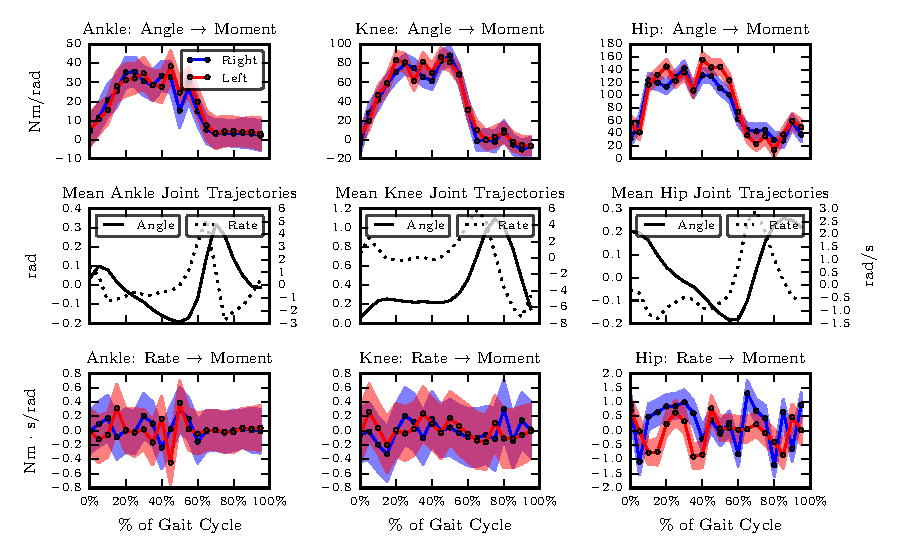
\includegraphics{figures/example-inverse-dynamics-correlation-gains.pdf}
    \caption{Gait phase percent scheduled gains for right (blue) and left (red) legs.}
    \label{fig:inverse-dynamics=correlation-gains}
  \end{center}
\end{figure}

The proportional gains show a clear bias that is strikingly similar to a
proportionally scaled vertical ground reaction force.

\subsection*{$\mathbf{m}^*$ accounts for most of the variation}
%
Ideally the variation in the gait cycles is sufficient to identify the
acutation due to feedback encapsulated by the gait matrix. If the feedback
contribution is assumed to be zero, then $\mathbf{m}^*$ can be identified
alone. If the VAF decreases significantly with $\mathbf{K}{\phi}=0$ then one
can assume that the feedback terms are not just contributing to overfitting the
data.
%
\begin{table}
  \cprotect\caption{Generated by \verb|src/table_no_control_vaf_comparison.py|.}
  \centering
  \begin{tabular}{lrrr}
\toprule
{} &  No Control &  Joint Isolated Control &  Full Control \\
\midrule
Left.Ankle.PlantarFlexion.Moment  &    0.930155 &                0.965969 &      0.974489 \\
Left.Hip.Flexion.Moment           &    0.930070 &                0.942240 &      0.968361 \\
Left.Knee.Flexion.Moment          &    0.841471 &                0.888560 &      0.935461 \\
Right.Ankle.PlantarFlexion.Moment &    0.943745 &                0.971717 &      0.979205 \\
Right.Hip.Flexion.Moment          &    0.965763 &                0.973759 &      0.984328 \\
Right.Knee.Flexion.Moment         &    0.810439 &                0.854908 &      0.901859 \\
\bottomrule
\end{tabular}

  \label{tab:no-control-vaf}
\end{table}

Table~\ref{tab:no-control-vaf} shows that $\mathbf{m}^*$ alone is sufficient to
explain a large portion of the variance in the data. Adding the feedback terms
pushes the VAF closer to 100\%.

\subsection*{Similar gains are predicted from both unperturbed and perturbed}
%

\section*{Discussion}
%
We are able to identify a simple linear controller that exhibits larger gains
in the stance phase than in the swing phase. Additionally, similar gain
patterns in the right and left legs are observed that use both positive and
negative feedback. The controller is capable of predicting the measured joint
torques with greater than 65\% VAF in all joints. Results and conclusions from
a larger sample of subjects and conditions will be presented at the conference.

\section*{Acknowledgments}

This research was funded by the Ohio's Wright Center for Sensor Systems
Engineering and the Parker Hannifin Corporation.

\end{document}
